\documentclass[11pt,a4paper]{article}
\usepackage[margin=1in]{geometry}
\usepackage{graphicx}
\usepackage{booktabs}
\usepackage{hyperref}
\usepackage{xcolor}
\usepackage{float}
\usepackage{amsmath}
\usepackage[font=small,labelfont=bf]{caption}

\hypersetup{colorlinks=true, linkcolor=blue!60!black, citecolor=blue!60!black, urlcolor=blue!60!black}

\title{\textbf{Marine Heatwave SST Scenarios for SSWD-EvoEpi}\\[0.5em]
\large Temperature Forcing Design for Evolutionary-Epidemiological Simulations}
\author{SSWD-EvoEpi Project}
\date{March 2025}

\begin{document}
\maketitle

\begin{abstract}
This report describes the design and construction of 12 synthetic sea surface temperature (SST) scenarios for marine heatwave (MHW) experiments in the SSWD evolutionary-epidemiological model. The scenarios are built from the real ``Pacific Blob'' (2013--2016) spatial anomaly fingerprint extracted from OISST data across 896 coastal monitoring sites spanning Baja California to the Aleutian Islands. Scenarios cover single events at three intensities, recurring events at four frequencies, ramping intensity, chronic warming, and compound events. All scenarios maintain the Blob's characteristic spatial gradient---strongest warming in the Gulf of Alaska, moderate along the open coast, and buffered in the Salish Sea.
\end{abstract}

\section*{Executive Summary}

\begin{itemize}
    \item \textbf{12 scenarios} generated, each containing 896 site-level monthly SST files spanning 2012--2050 (468 months per site).
    \item \textbf{Blob template} extracted from 2014--2016 anomalies vs.\ 2002--2012 monthly climatology. Peak anomaly (2015) averages +1.4$^\circ$C coast-wide, with values exceeding +2$^\circ$C in Alaska.
    \item \textbf{Heatwave lifecycle} uses a compressed 24-month pattern: 6-month onset $\rightarrow$ 12-month peak $\rightarrow$ 6-month dissipation, preserving the Blob's temporal structure.
    \item \textbf{Key comparison axes}: intensity (0.5$\times$--1.5$\times$), frequency (3--10 year return), and chronic vs.\ pulsed warming.
    \item All temperatures capped at 30$^\circ$C. Pre-2025 data uses original OISST observations.
\end{itemize}

\section{Blob Template Analysis}

The Pacific Blob was a persistent marine heatwave that affected the northeast Pacific from 2013 to 2016. We extract its spatial-temporal fingerprint from our OISST monitoring network to serve as the template for all heatwave scenarios.

\subsection{Temporal Structure}

Figure~\ref{fig:blob_template} shows the monthly anomaly patterns for 2014 (onset year), 2015 (peak year), and 2016 (dissipation year), aggregated by region from south (Baja California) to north (Aleutian Islands).

\begin{figure}[H]
    \centering
    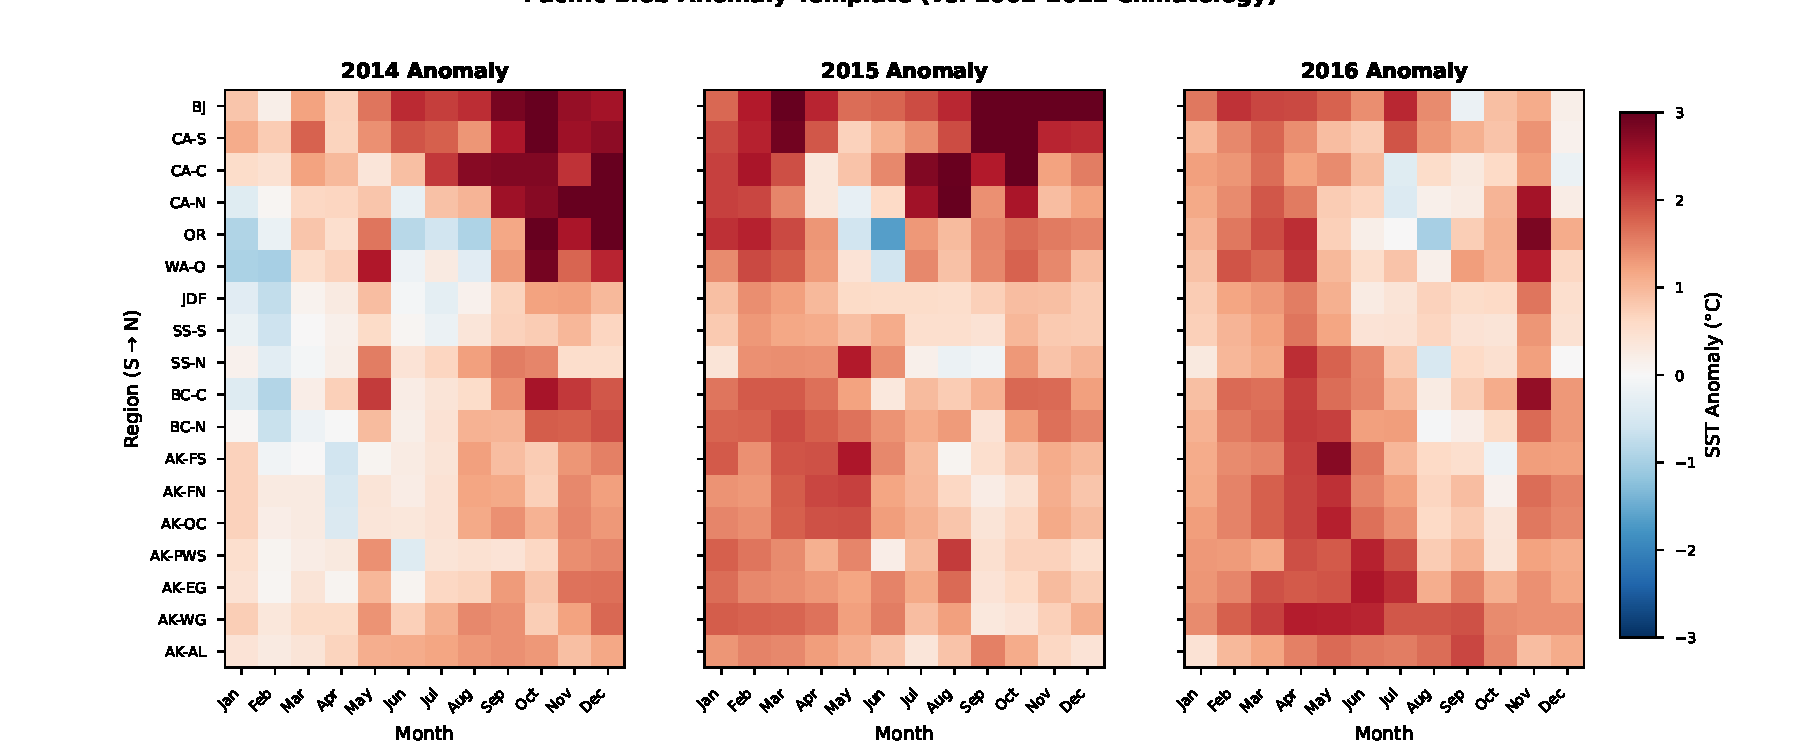
\includegraphics[width=\textwidth]{figures/fig_blob_template.pdf}
    \caption{\textbf{Pacific Blob anomaly template.} Monthly SST anomalies (vs.\ 2002--2012 climatology) for 2014, 2015, and 2016, averaged by region and ordered south to north. The Blob intensified through 2014, peaked in 2015 with anomalies exceeding +2--3$^\circ$C in Alaska, and dissipated through 2016. Note the persistent positive anomalies across all regions and months, with strongest warming in summer--fall.}
    \label{fig:blob_template}
\end{figure}

\subsection{Spatial Gradient}

The Blob's spatial structure is a critical feature: warming was strongest at higher latitudes, particularly in the Gulf of Alaska, while the Salish Sea experienced more moderate anomalies due to topographic buffering.

\begin{figure}[H]
    \centering
    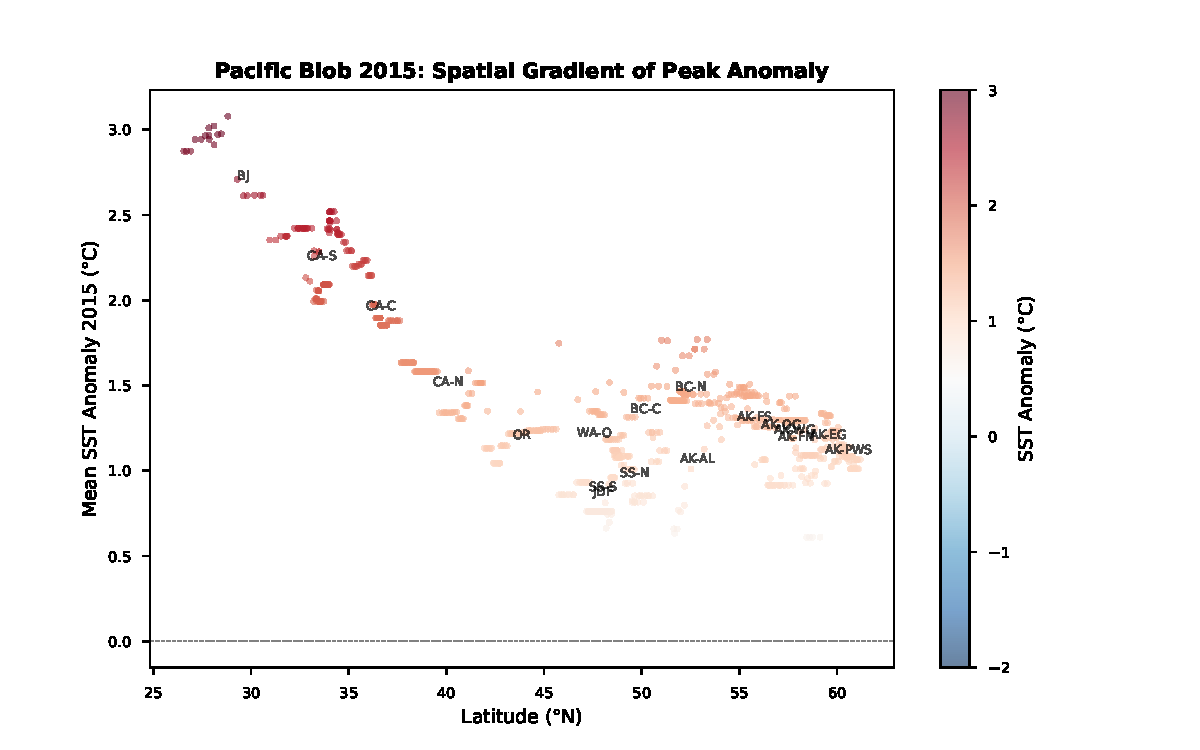
\includegraphics[width=0.85\textwidth]{figures/fig_blob_spatial.pdf}
    \caption{\textbf{Latitudinal gradient of peak Blob anomaly (2015).} Each point represents one of 896 monitoring sites, colored by anomaly magnitude. The gradient shows stronger warming at higher latitudes (50--60$^\circ$N), with the Salish Sea sites (48--49$^\circ$N) showing notably reduced anomalies relative to their latitude. This spatial heterogeneity is naturally preserved in all scenarios since we use the actual Blob fingerprint as the template.}
    \label{fig:blob_spatial}
\end{figure}

\section{Scenario Design}

Twelve scenarios explore three axes of variation: event intensity, recurrence frequency, and warming pattern (pulsed vs.\ chronic).

\begin{table}[H]
\centering
\small
\begin{tabular}{llcll}
\toprule
\textbf{ID} & \textbf{Description} & \textbf{Intensity} & \textbf{Event Years} & \textbf{Notes} \\
\midrule
MHW\_CTRL & Control & --- & --- & No heatwave \\
MHW\_S1\_LOW & Single, moderate & 0.5$\times$ & 2030 & Half-Blob \\
MHW\_S1\_MED & Single, Blob-like & 1.0$\times$ & 2030 & Exact replay \\
MHW\_S1\_HIGH & Single, extreme & 1.5$\times$ & 2030 & 50\% amplified \\
\midrule
MHW\_R10\_MED & Recurring 10yr & 1.0$\times$ & 2030, 2040, 2050 & Conservative \\
MHW\_R7\_MED & Recurring 7yr & 1.0$\times$ & 2028, 2035, 2042, 2049 & Moderate \\
MHW\_R5\_MED & Recurring 5yr & 1.0$\times$ & 2028, 2033, 2038, 2043, 2048 & Frequent \\
MHW\_R5\_HIGH & Recurring 5yr, intense & 1.5$\times$ & 2028, 2033, 2038, 2043, 2048 & Worst case \\
MHW\_R3\_MED & Recurring 3yr & 1.0$\times$ & 8 events, 2028--2049 & Very frequent \\
\midrule
MHW\_RAMP & Intensifying & 0.5$\rightarrow$1.5$\times$ & 2028, 2033, 2038, 2043, 2048 & Progressive \\
MHW\_CHRONIC & Permanent +1$^\circ$C & --- & 2025+ & Background warming \\
MHW\_COMPOUND & Back-to-back & 1.0$\times$ & 2030 (36-mo) + 2033 (24-mo) & No recovery \\
\bottomrule
\end{tabular}
\caption{Summary of 12 marine heatwave SST scenarios.}
\label{tab:scenarios}
\end{table}

\subsection{All Scenarios at a Glance}

\begin{figure}[H]
    \centering
    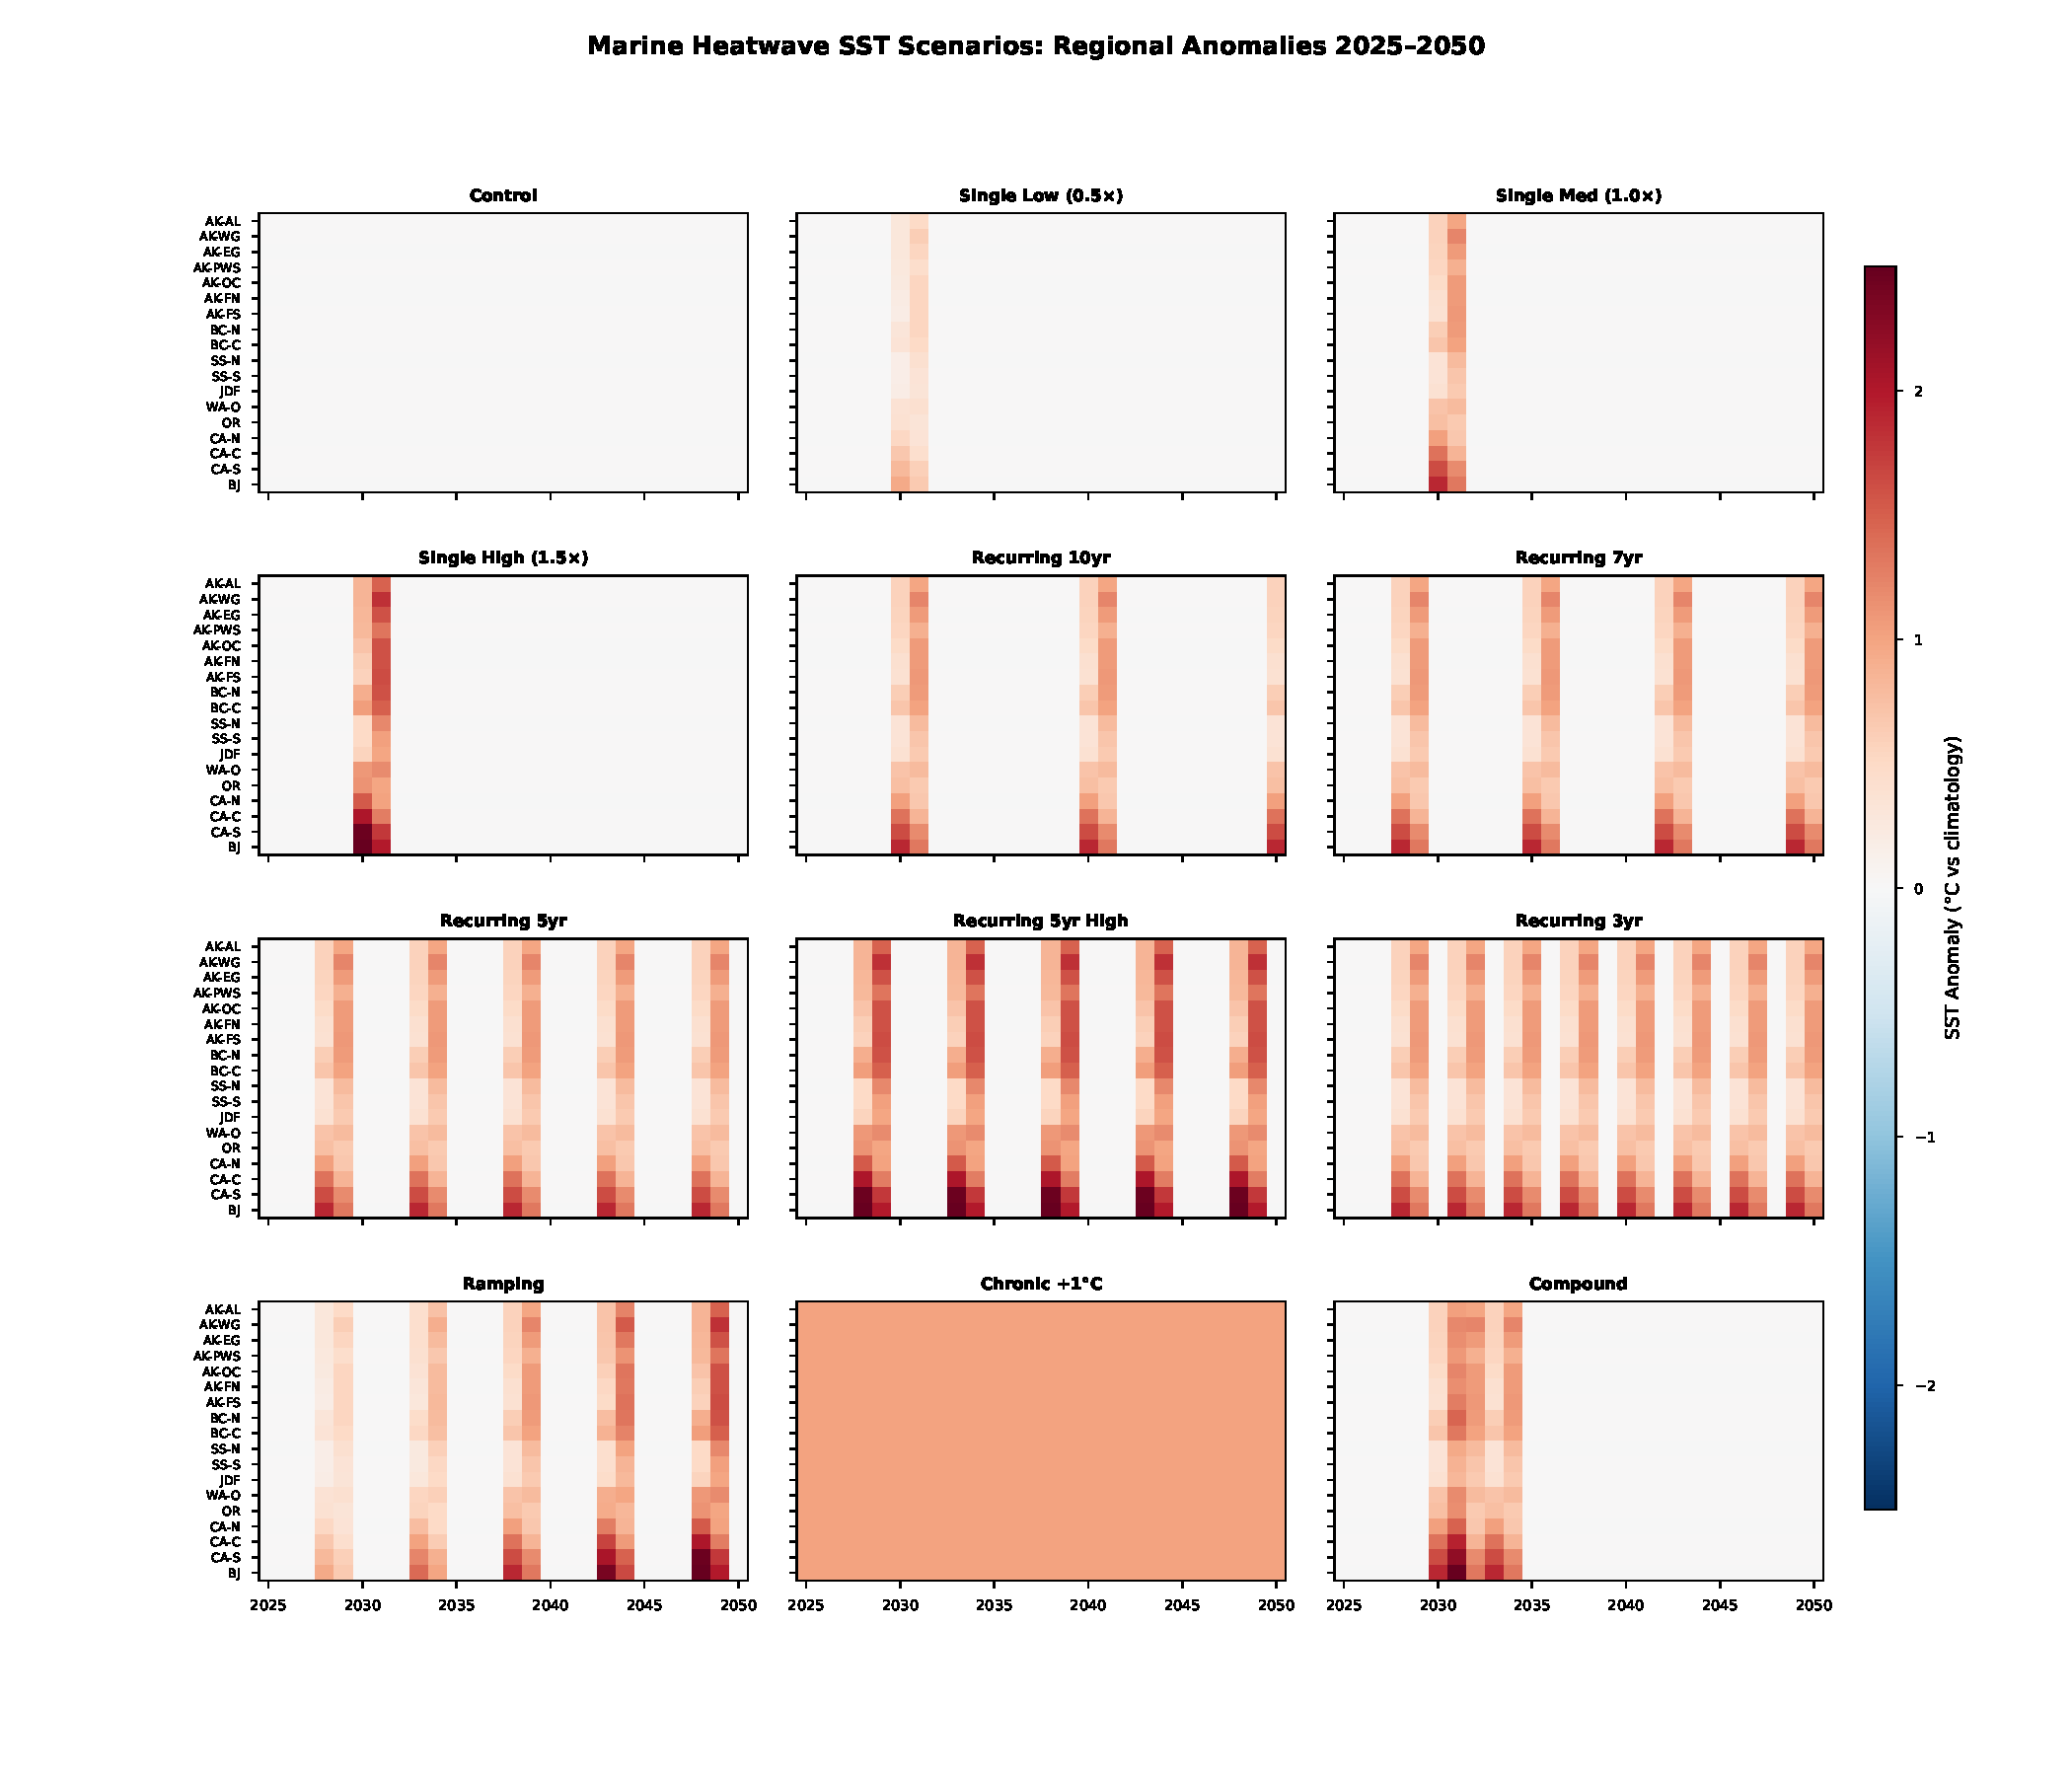
\includegraphics[width=\textwidth]{figures/fig_scenario_comparison.pdf}
    \caption{\textbf{Marine heatwave scenario comparison (hero figure).} Each panel shows the regional mean SST anomaly (vs.\ 2002--2012 climatology) for one scenario, with regions ordered south to north (y-axis) and time on the x-axis (2025--2050). Red indicates warming above climatology. The Control panel (top left) shows zero anomaly by construction. Recurring scenarios show periodic warming pulses; the Chronic scenario shows uniform +1$^\circ$C; the Compound scenario shows overlapping events with no recovery period. All panels share the same color scale for direct comparison.}
    \label{fig:scenario_comparison}
\end{figure}

\subsection{Intensity Comparison}

\begin{figure}[H]
    \centering
    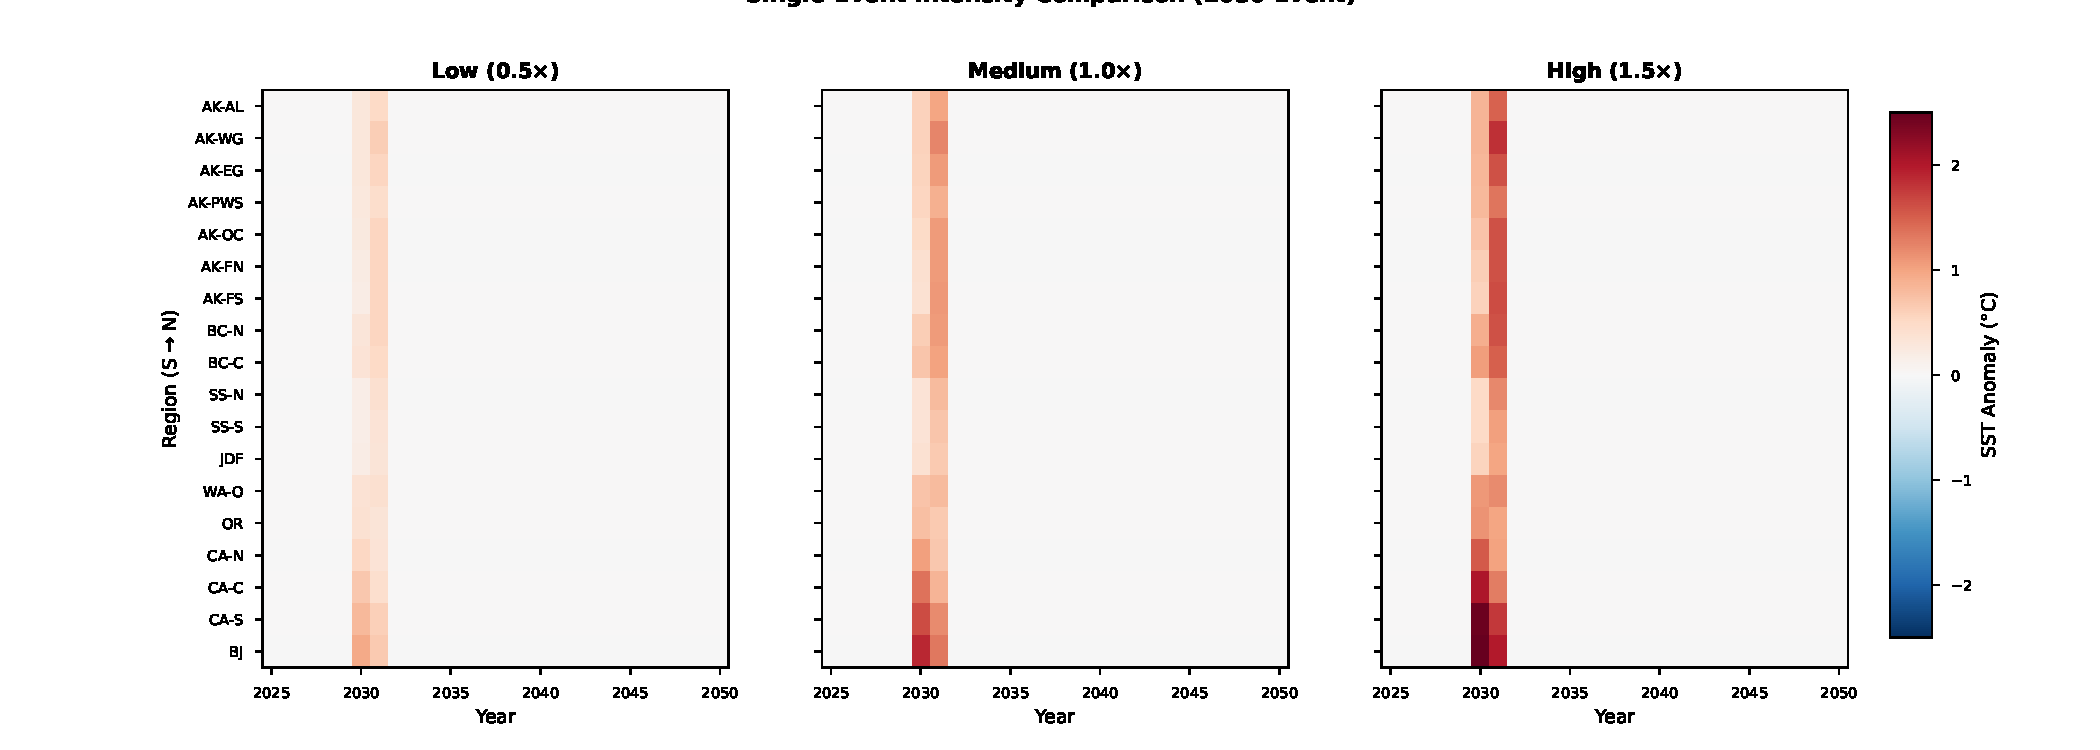
\includegraphics[width=\textwidth]{figures/fig_intensity_comparison.pdf}
    \caption{\textbf{Single-event intensity comparison.} Three panels showing the same 2030 heatwave event at 0.5$\times$ (Low), 1.0$\times$ (Medium, Blob-equivalent), and 1.5$\times$ (High) intensity. The spatial pattern is identical across panels---only the magnitude scales. At 1.5$\times$, peak anomalies in Alaska exceed +3$^\circ$C.}
    \label{fig:intensity}
\end{figure}

\subsection{Frequency Comparison}

\begin{figure}[H]
    \centering
    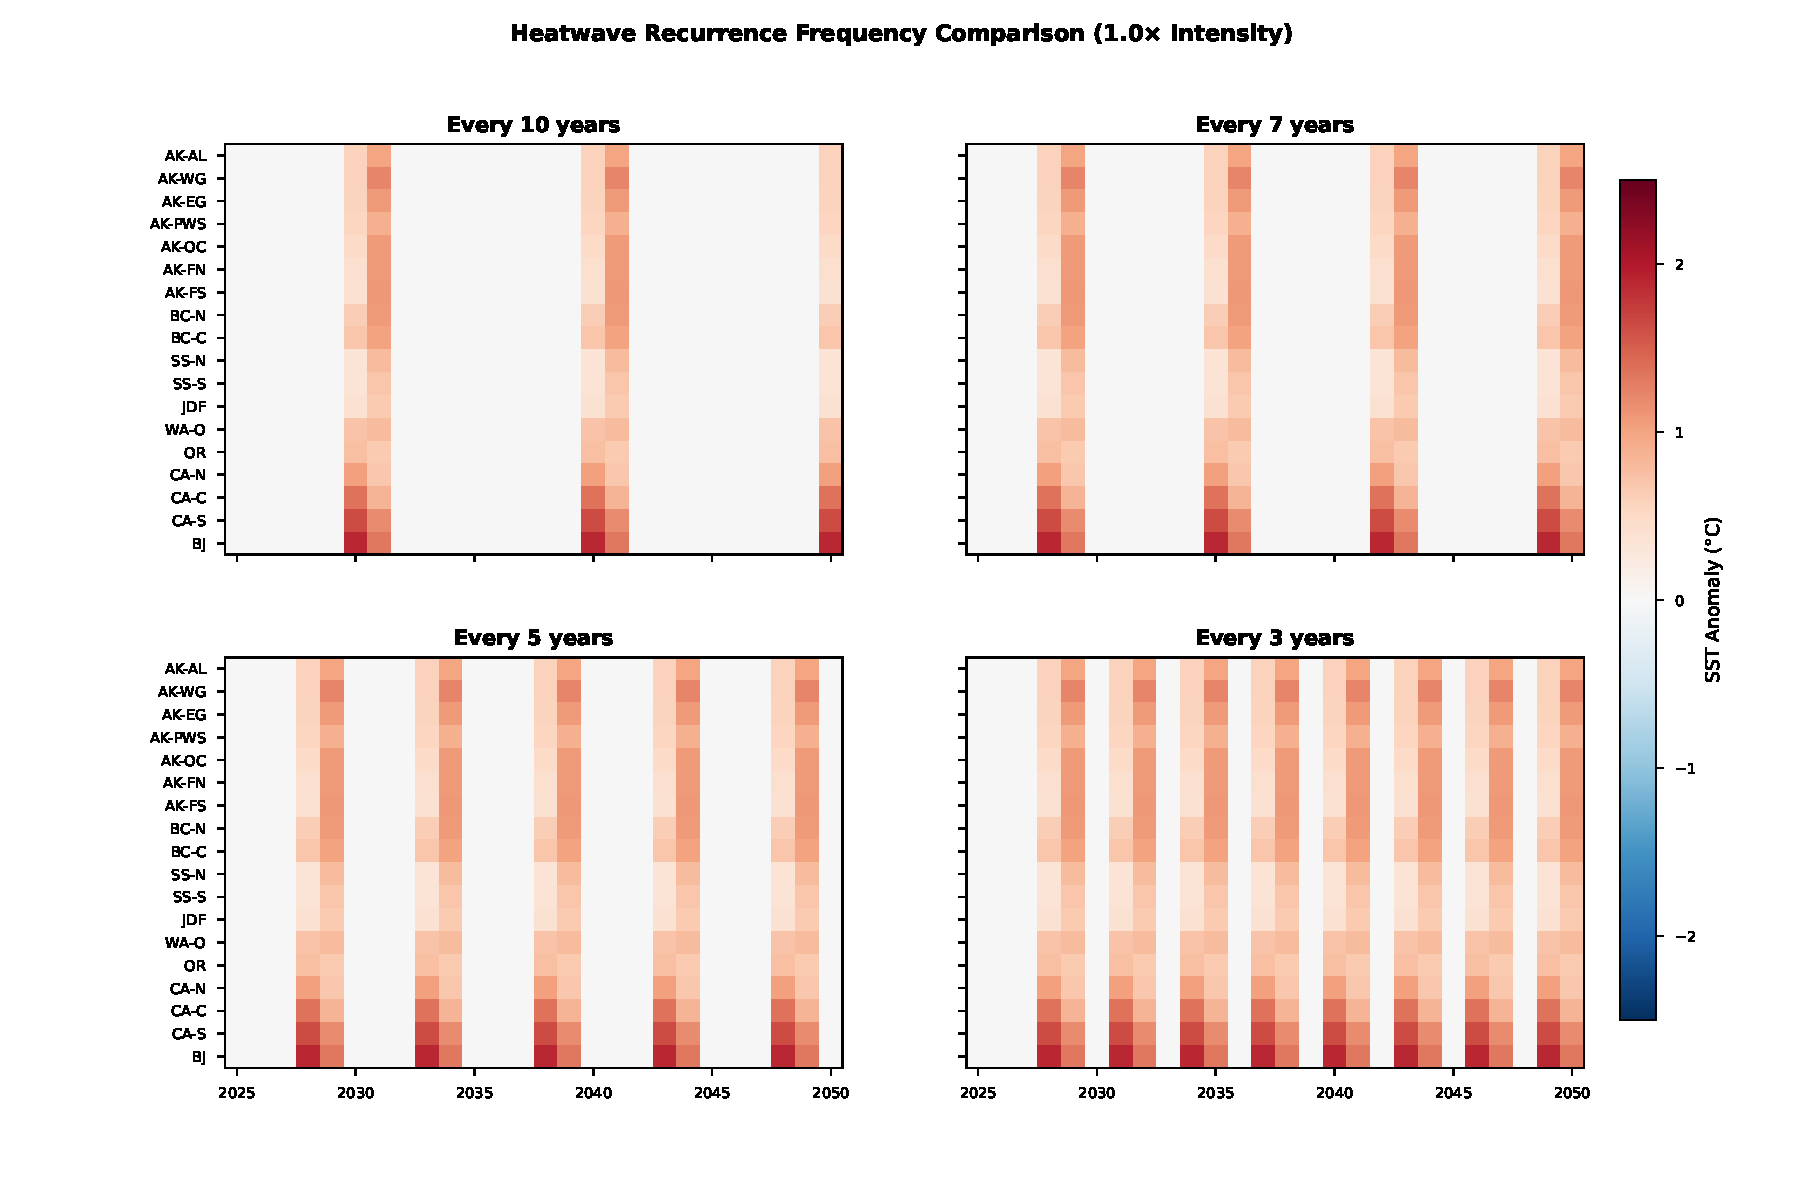
\includegraphics[width=\textwidth]{figures/fig_frequency_comparison.pdf}
    \caption{\textbf{Recurrence frequency comparison.} Four panels showing heatwave events recurring every 10, 7, 5, and 3 years at 1.0$\times$ (Blob-equivalent) intensity. At 3-year recurrence, events overlap significantly since each event spans 24 months, leaving minimal recovery time between events.}
    \label{fig:frequency}
\end{figure}

\section{Regional Detail}

\subsection{SST Trajectories}

\begin{figure}[H]
    \centering
    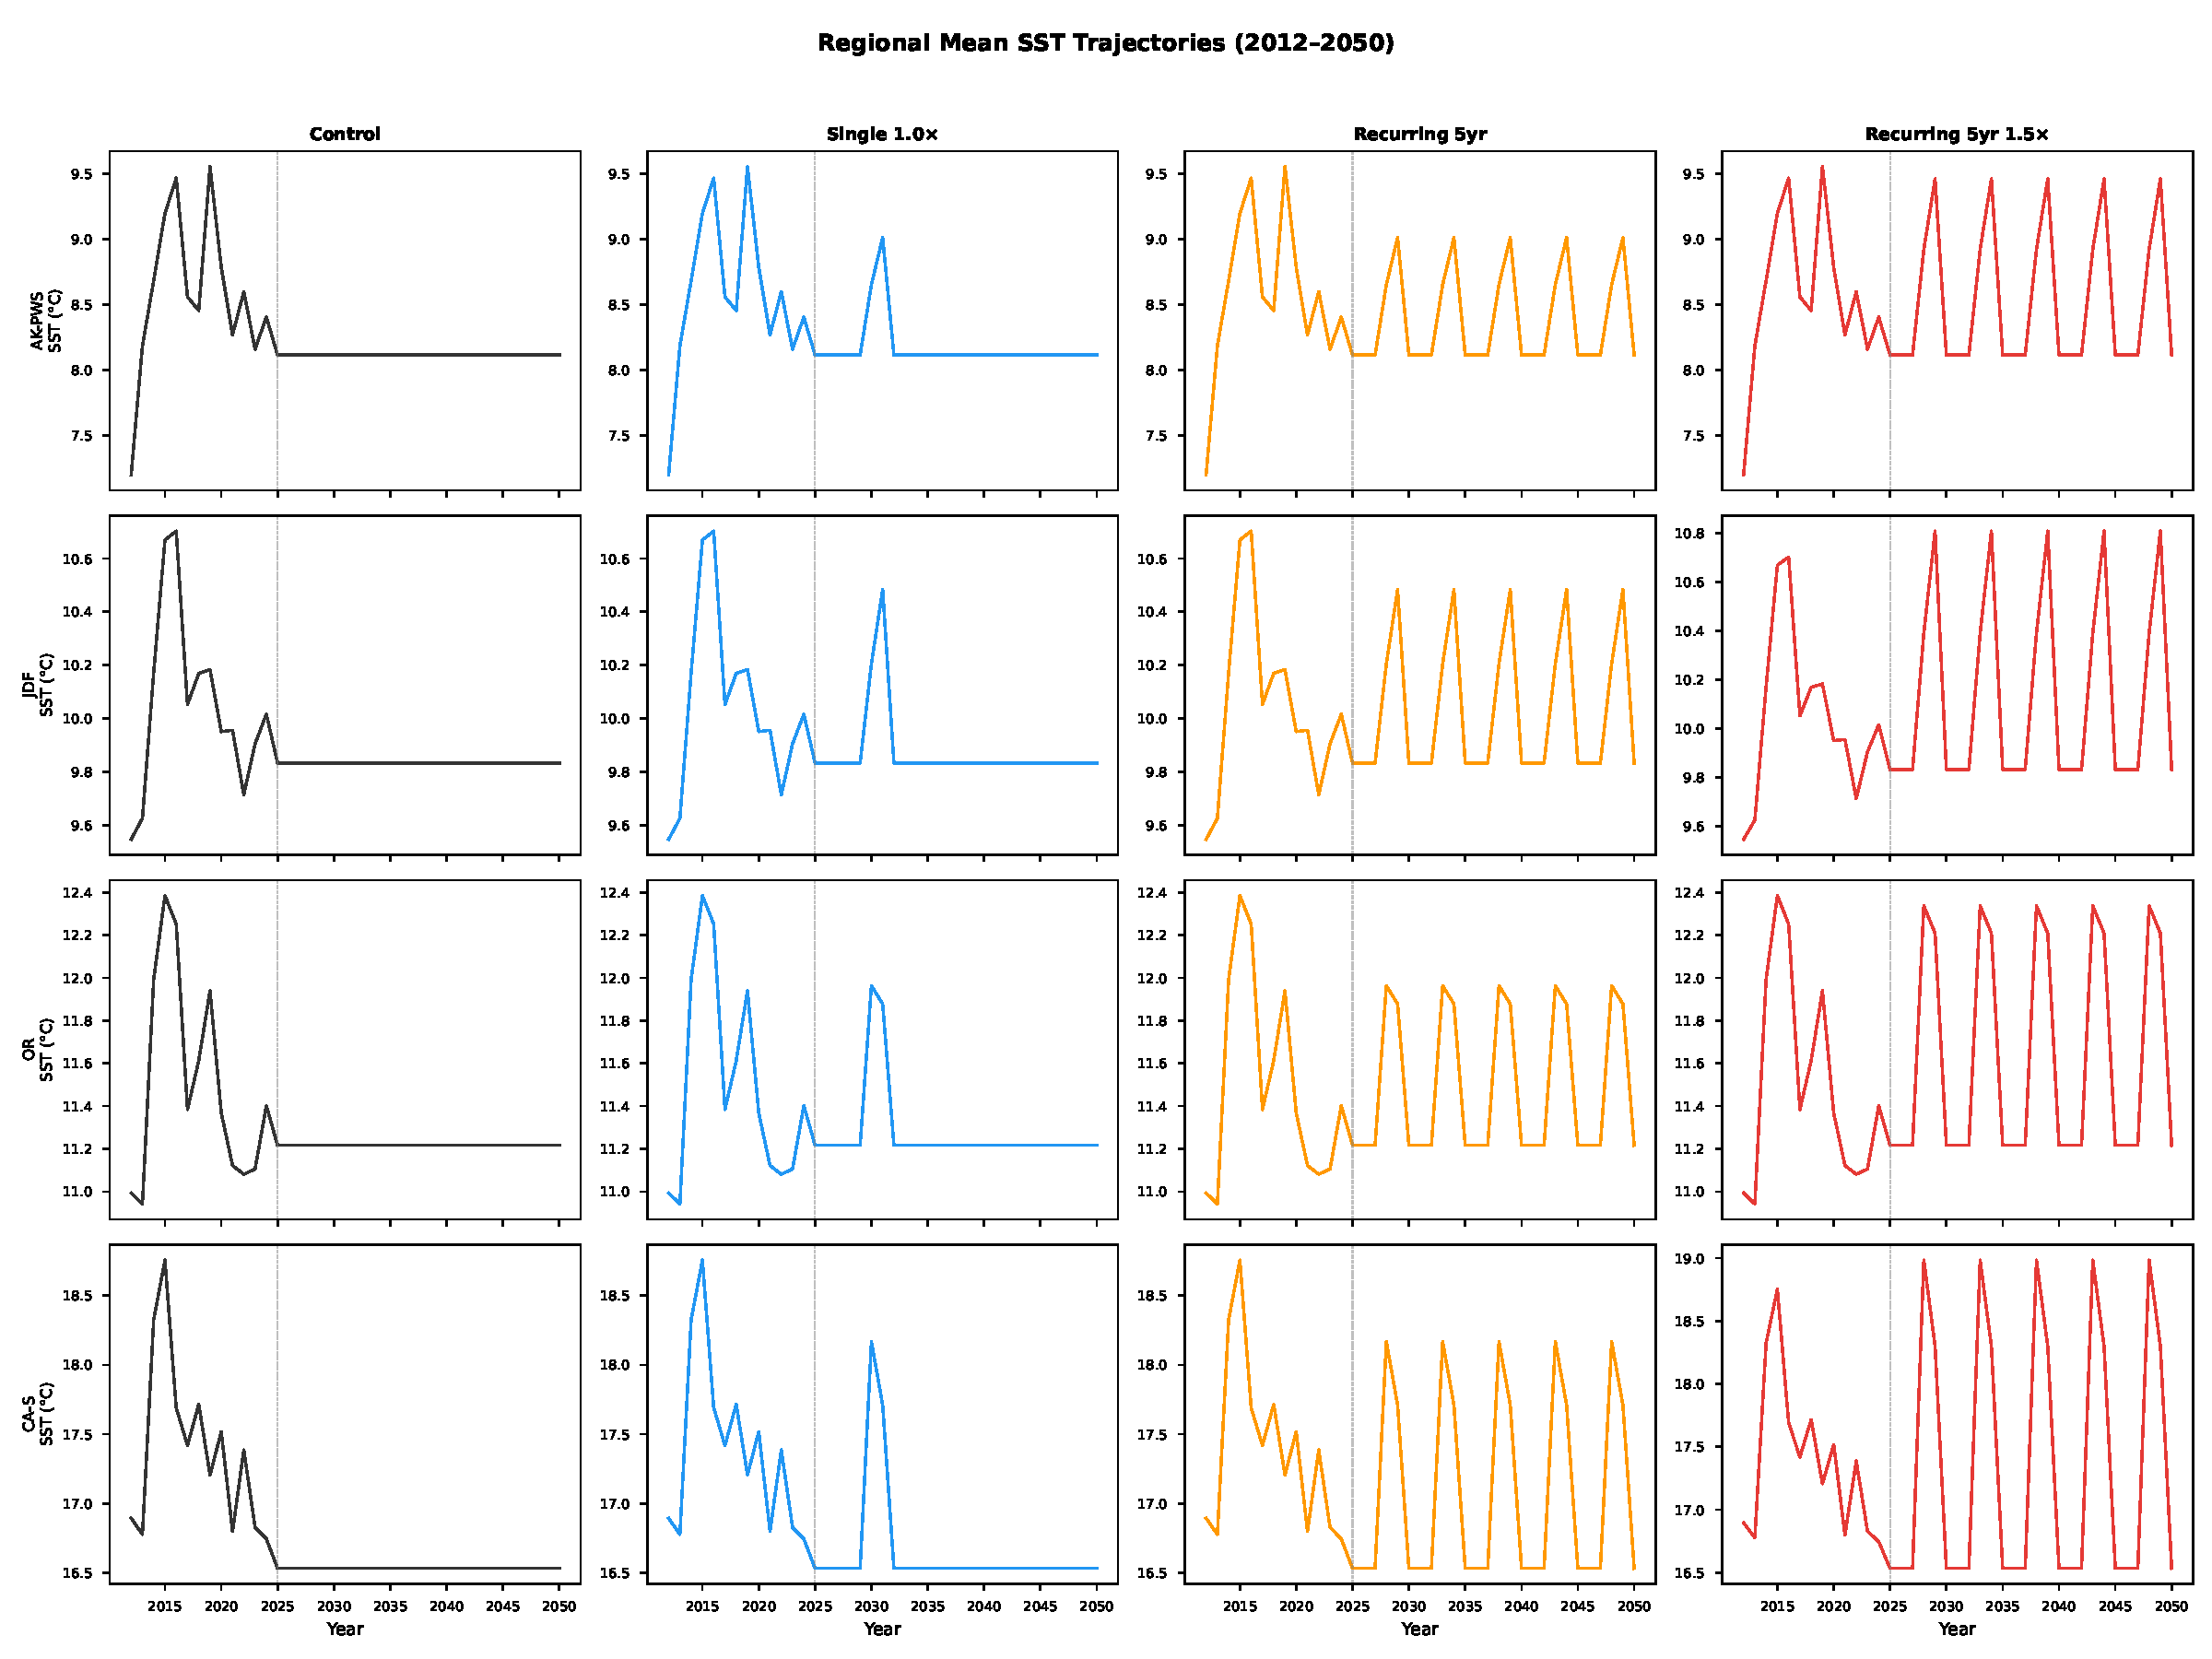
\includegraphics[width=\textwidth]{figures/fig_regional_sst_timeseries.pdf}
    \caption{\textbf{Regional mean SST time series (2012--2050).} Four representative regions (AK-PWS, JDF, OR, CA-S) under four scenarios. The vertical dashed line marks 2025, where synthetic SST begins. Pre-2025 trajectories are identical (original OISST data). Post-2025, the Control scenario uses flat climatology, while heatwave scenarios show characteristic warming pulses.}
    \label{fig:timeseries}
\end{figure}

\subsection{Simulated vs.\ Real Blob}

\begin{figure}[H]
    \centering
    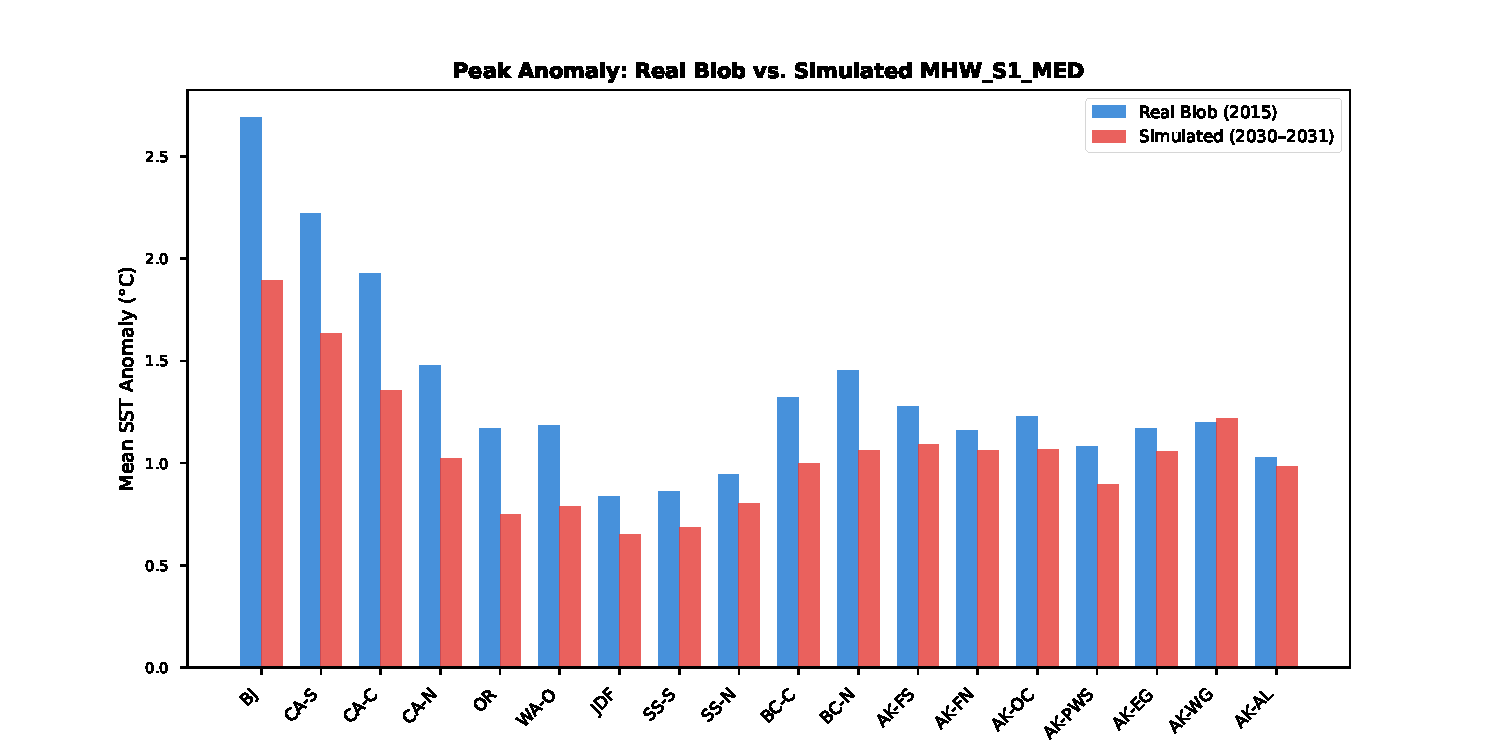
\includegraphics[width=0.85\textwidth]{figures/fig_peak_anomaly_map.pdf}
    \caption{\textbf{Peak anomaly comparison: real Blob (2015) vs.\ simulated event (MHW\_S1\_MED, 2030--2031).} The simulated event closely reproduces the real Blob's regional pattern, including the characteristic amplification in Alaska and buffering in the Salish Sea. Minor differences arise from the temporal compression (24-month lifecycle vs.\ the Blob's actual multi-year evolution).}
    \label{fig:peak_anomaly}
\end{figure}

\subsection{Chronic vs.\ Pulsed Warming}

\begin{figure}[H]
    \centering
    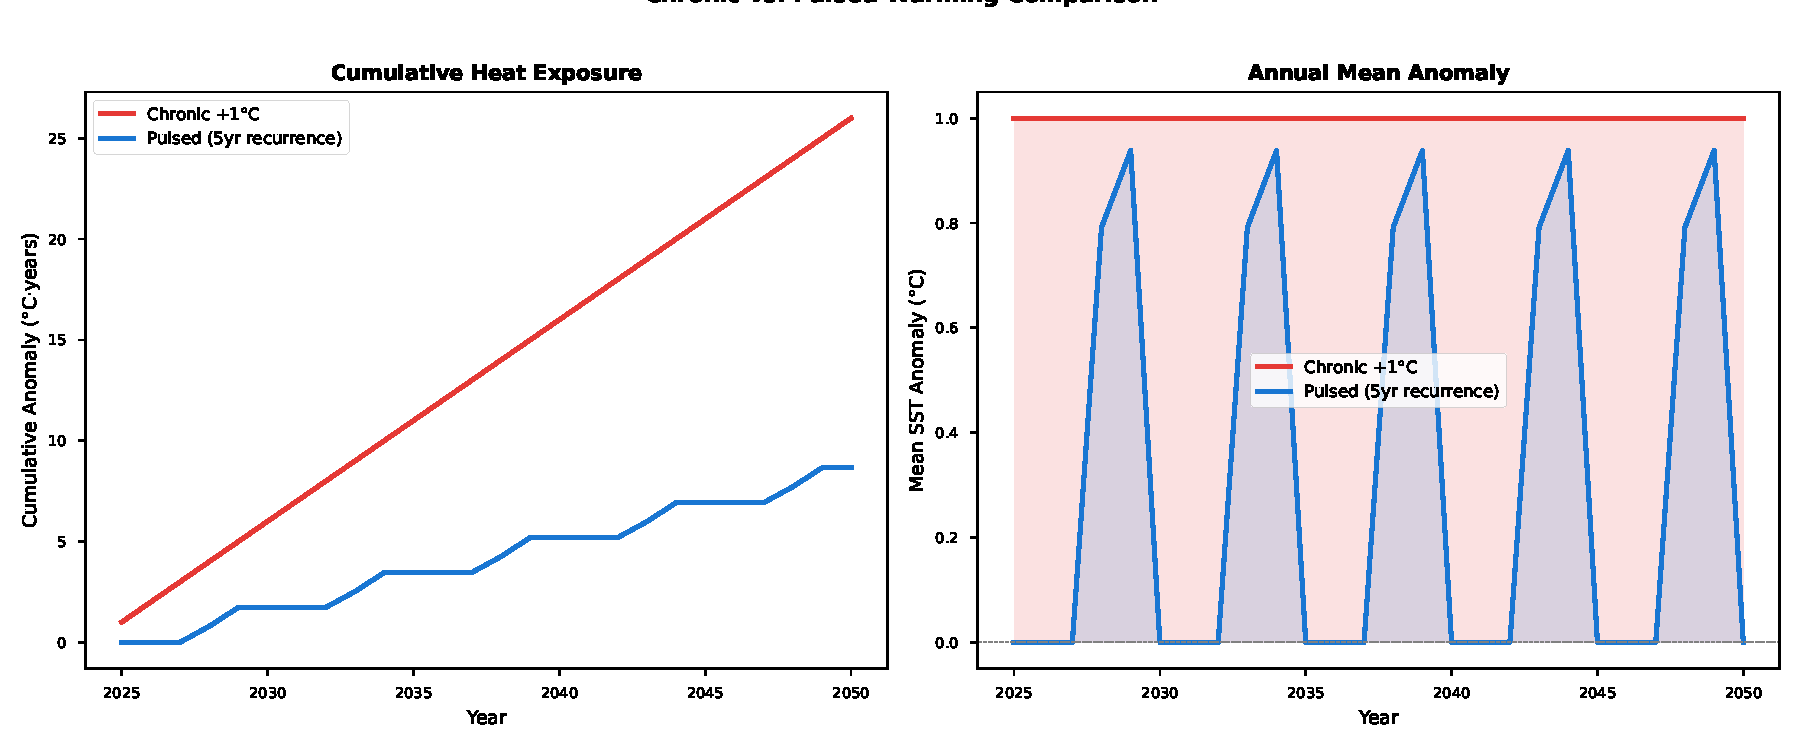
\includegraphics[width=\textwidth]{figures/fig_chronic_vs_pulse.pdf}
    \caption{\textbf{Chronic vs.\ pulsed warming comparison.} Left: cumulative heat exposure over 2025--2050. The chronic +1$^\circ$C scenario accumulates heat steadily, while the pulsed scenario (5-year recurrence) shows stepwise increases during events. Right: annual mean anomaly showing the contrasting temporal patterns. Despite similar cumulative exposure, the ecological impact may differ---chronic warming allows adaptation, while pulsed events may overwhelm thermal tolerance.}
    \label{fig:chronic_pulse}
\end{figure}

\section*{Technical Notes}

\begin{itemize}
    \item \textbf{Baseline climatology}: 2002--2012 monthly mean SST per site (11-year average).
    \item \textbf{Pre-2025 data}: Original OISST observations used unchanged.
    \item \textbf{Post-2025 construction}: Climatology + scaled Blob anomalies during event windows.
    \item \textbf{Temperature cap}: All SST values capped at 30$^\circ$C.
    \item \textbf{Heatwave lifecycle}: 24-month compressed pattern using 2014 (onset), 2015 (peak), and 2016 (dissipation) anomaly templates with 0.5$\times$/1.0$\times$/0.5$\times$ scaling.
    \item \textbf{Site count}: 896 monitoring sites across 18 regions (BJ to AK-AL).
    \item \textbf{Temporal extent}: 2012--2050 (39 years, 468 monthly timesteps per site).
\end{itemize}

\end{document}
